\section*{Аннотация}

\subsection*{Цель работы}
Познакомиться с явлением интерференции в тонких
плёнках (полосы равной толщины) на примере колец Ньютона и с
методикой интерференционных измерений кривизны стеклянной поверхности.
\section*{Теоретические сведения}
\indent Кольца Ньютона представляют собой интерференцию волн, отражённых от границ тонкой 
воздушной прослойки, образованной сферической поверхностью линзы и плоской
стеклянной пластиной. При нормальном падении света интерференционные полосы 
локализованы на сферической поверхности и являются полосами равной толщины.

\begin{wrapfigure}{l}{0.3\linewidth}
    \centering
    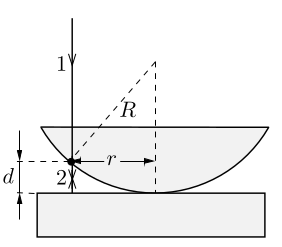
\includegraphics[width=4cm]{images/theory.png}
    \caption{Схема наблюдения колец Ньютона}
\end{wrapfigure}

\indent
Найдем оптическую разность хода интерферирующих лучей. C учетом того, что $R \gg d$:
$$r^2 = R^2 - (R - d)^2 \approx 2Rd \quad \Rightarrow \quad d = \frac{r^2}{2R}$$ 
Тогда выражение для разности хода лучей с учетом потери полуволны при отражении от оптически более плотной среды:
\begin{equation}
    \Delta = 2d + \frac{\lambda}{2} = \frac{r^2}{R} + \frac{\lambda}{2}
\end{equation}
Условие интерференционного минимума:
\begin{equation}
    \Delta = (2m + 1)\frac{\lambda}{2}
\end{equation}
Отсюда получаем радиус темных и светлых колец соответственно:
\begin{equation}
    r_m = \sqrt{m\lambda R}
\end{equation}

\begin{equation}
    r_m' = \sqrt{(2m - 1)\lambda R/ 2}
\end{equation}

\newpage
\section*{Экспериментальная установка}
\textbf{Оборудование:} \textit{измерительный микроскоп с опак-иллюминатором; плосковыпуклая линза; пластинка из чёрного стекла;
ртутная лампа ДРШ; щель; линзы; призма прямого зрения; объектная шкала.}

\begin{figure}[h!]
    \centering
    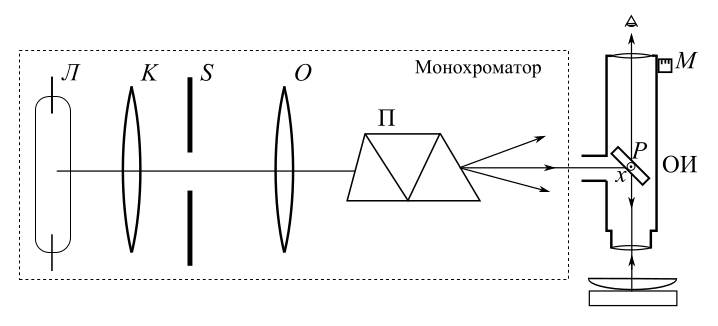
\includegraphics[width=12cm]{images/setup.png}
    \caption{Схема экспериментальной установки}
\end{figure}

Опыт выполняется с помощью измерительного микроскопа. На столике микроскопа  
помещается держатель с пластинкой чёрного стекла. На пластинке лежит 
исследуемая линза.
Источником света служит ртутная лампа, находящаяся в защитном кожухе. Для получения монохроматического света применяется
призменный монохроматор, состоящий из конденсора K, коллиматора (щель S и объектив O) и призмы прямого зрения П. Эти устройства с помощью рейтеров располагаются на оптической скамье. Свет от
монохроматора попадает на опак-иллюминатор (ОИ), расположенный
между окуляром и объективом микроскопа - специальное устройство
для освещения объекта при работе в отражённом свете. Внутри опак-иллюминатора находится полупрозрачная пластинка P , наклоненная
под углом $45^{\circ}$ к оптической оси микроскопа. Свет частично отражается от этой пластинки, проходит через объектив микроскопа и попадает
на исследуемый объект. Пластинка может поворачиваться вокруг горизонтальной оси x, а опак-иллюминатор — вокруг вертикальной оси.


\section*{Ход работы}
\subsection*{Определение радиуса кривизны линзы}
\subsection*{Наблюдение биений}
\subsection*{Калибровка окулярной оси}

\section*{Вывод}





